\documentclass[a4paper,oneside]{Tptesi2}

\usepackage[italian]{babel}
\usepackage{listings}
\usepackage{amsmath,amssymb}
\usepackage{verbatim}
\usepackage{indentfirst}
\usepackage[utf8]{inputenc}
%\usepackage{subfigure}
\usepackage{algorithmic} 
\usepackage{framed}
\usepackage{rotating}
\usepackage[superscript]{cite}
\usepackage{subfig}

% Packages -----------------------------------------------------------------------
\renewcommand\citeform[1]{[#1]}


% Use a small font for the verbatim environment
\makeatletter  % makes '@' an ordinary character
\renewcommand{\verbatim@font}{%
  \ttfamily\footnotesize\catcode`\<=\active\catcode`\>=\active%
}
\makeatother   % makes '@' a special symbol again
%
% Simboli Matematici -------------------------------------------------------------
%\newcommand{\h}{\mathcal{H}_\infty} % scorciatoia per sequenza usata spesso
% Definizioni & Teoremi ----------------------------------------------------------
\newtheorem{teorema}{Teorema}[chapter]
\newtheorem{corollario}[teorema]{Corollario} 
\newtheorem{lemma}[teorema]{Lemma}
%\theoremstyle{definition}
\newtheorem{definizione}{Definizione}[chapter]
\newtheorem{proposizione}[definizione]{Proposizione}
% Formattazione Figure -----------------------------------------------------------
\setcounter{topnumber}{3}
\setcounter{totalnumber}{3}
\def\topfraction{1}
\def\textfraction{0}
% Fuzz ---------------------------------------------------------------------------
%\hfuzz10cm %Non scassare linee che escono dal bordo
% Frontespizio -------------------------------------------------------------------
       \title{Title...}
       \author{Lorenzo Niccolai}
       \titolocorso{Ingegneria Informatica}
       \chair{Prof. Enrico Vicario \\ }
       \numberofmembers{1} %numero dei relatori
       \degreeyear{2019/2020}
       \numerocorrelatori{1} %numero dei correlatori
       \correlatori{???} % i correlatori separati da \\

\hypersetup{%
%  pdfpagemode=FullScreen,%
  plainpages=false,%
  breaklinks,%
  pdftitle={},%
  pdfauthor={},%
  pdfsubject={},%
  pdfkeywords={},%
  colorlinks=false}

\begin{document}

\frontmatter

\pagestyle{headings}

\maketitle

\tableofcontents

\cleardoublepage


%\pagenumbering{arabic}
%\input{files/ringraziamenti}
\frontmatter
\chapter{Introduzione}\label{ch:introduzione}
%\cite{gruntzig1978transluminal}
L'obiettivo di questo lavoro è esporre un servizio su cloud in forma di \textit{software as a service} che implementi una 
funzione basata su Oris nel contesto del intelligent transportation per tramvie.

Sarà progettata e realizzata una moderna applicazione a servizi che implementa una serie di casi d'uso, e successivamente verrà proposta una metodologia che guida la rifattorizzazione di tale software verso la forma di microservizi, applicando a vari livelli il proncipio di "separazione delle responsabilità".

Sarà inoltre posta attenzione a varie tecnologie che potrebbero essere adottate nelle fasi di progettazione, sviluppo e rilascio.

\mainmatter
\chapter{Applicazione}

In questo capitolo saranno esposti i requisiti dell'applicazione, seguiti da una breve analisi e progettazione di un sistema che li implementa.

\section{Requisiti}
L'obiettivo principale è quello di poter definire e analizzare modelli virtuali di incrocio stradale, in modo da riuscire ad effettuare aggiustamenti sul traffico e quindi minimizzare l'impatto che può avere un mezzo come la tramvia sulla circolazione degli altri veicoli.

Per mantenere generale l'applicazione, dovrà essere possibile la descrizione di porzioni più ampie di mappa stradale in modo da supportare analisi di tipo diverso, nonché eventuali simulazioni.

In questo lavoro saranno realizzate le seguenti analisi esemplificative:
\begin{itemize}
	\item Disponibilità di un incrocio: la probabilità che le auto siano libere di procedere, ovvero che il semaforo sia verde.
	\item Lunghezza media di una coda: Considerando alcuni fattori come il tempo di attraversamento, si vuol sapere quale sarà la dimensione della coda delle auto.
	\item Tasso di overflow: Caso in cui un'auto non riesce ad entrare nella via a causa del traffico eccessivo.
\end{itemize}

Tramite il software sarà possibile definire, oltre alla topologia della rete stradale, una serie di parametri necessari all'analisi di essa.
Alcuni dei valori gestiti saranno:
\begin{itemize}
	\item Periodo dell'analisi: cadenza con la quale i treni arrivano in prossimità dell'incrocio;
	\item Eventuale ritardo di arrivo del tram;
	\item Tasso di arrivo delle auto;
	\item Tempo di attraversamento delle auto;
	\item Dimensione massima della coda (calcolabile dalla lunghezza del tratto di strada e dalla dimensione dei veicoli);
	\item Tempo di attraversamento del tram;
	\item Tempo di anticipo del semaforo rispetto all'arrivo; effettivo del treno;
\end{itemize}

Sempre con lo scopo di supportare analisi non ancora stabilite, sarà possibile impostare sui vari elementi della rete un numero arbitrario di parametri.
Questi saranno suggeriti dagli stessi moduli di analisi.


\section{Casi d'uso}

Sono state individuate tre categorie di utilizzatori (vedi figura \ref{fig:uc-users}):
\begin{itemize}
	\item Amministratore
	\item Esperto
	\item Cliente
\end{itemize}

\begin{figure}[h]
	\centering
	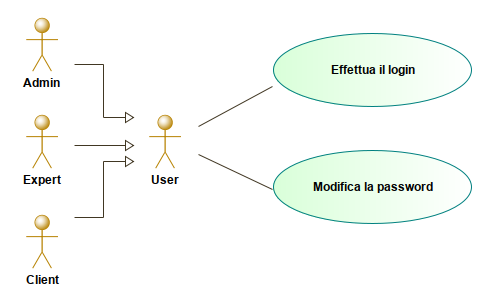
\includegraphics[scale=0.5]{img/UserUC}
	\caption{Classificazione degli utenti}
	\label{fig:uc-users}
\end{figure}

Ogni utente potrà accedere all'applicazione tramite una funzionalità di login, così da avere accesso alle aree del software di propria competenza, nonchè alla sezione di gestione del profilo.

Gli utenti di tipo \textit{amministratore} hanno la possibilità di gestire gli accounts aggiungendone di nuovi o eliminandone di esistenti (figura \ref{fig:uc-admins}).
Per semplicità sarà lo stesso amministratore a stabilire le password iniziali, che potranno essere modificate in seguito dai proprietari.

\begin{figure}[h]
	\centering
	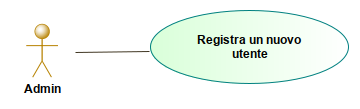
\includegraphics[scale=0.5]{img/AdminUC}
	\caption{Casi d'uso di un amministratore}
	\label{fig:uc-admins}
\end{figure}

Gli utenti \textit{esperti} conoscono a fondo il dominio e sono in grado di configurare un modello specificando le varie proprietà.
Per questo hanno il permesso di definire valori di default o complete configurazioni per gli utenti meno esperti (figura \ref{fig:uc-experts}).

\begin{figure}[h]
	\centering
	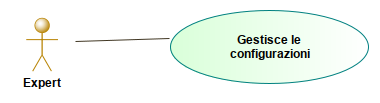
\includegraphics[scale=0.5]{img/ExpertUC}
	\caption{Casi d'uso di un utente esperto}
	\label{fig:uc-experts}
\end{figure}

Gli utenti semplici possono creare dei progetti personali.
Questi raggruppano una serie di topologie di rete.
Una volta creata e validata una mappa, sarà possibile lanciare delle analisi che rimarranno legate ad essa e delle quali sarà possibile monitorare lo stato ed accedere ai risultati.

In figura \ref{fig:cd-conceptual} è mostrato un semplice diagramma concettuale che sarà poi raffinato nelle fasi successive.
\'E possibile apprezzare le relazioni tra le varie entità nominate precedentemente.

\begin{figure}[h]
	\centering
	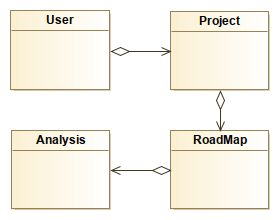
\includegraphics[scale=0.5]{img/conceptual00}
	\caption{Schema concettuale}
	\label{fig:cd-conceptual}
\end{figure}



\section{Modellazione della rete stradale}
Interesse di questo lavoro è lo studio del traffico nei pressi di un incrocio tra auto e tramvia.
Per supportare una visione più ampia, ed altre eventuali tipologie di analisi, sarà proposto un modello in grado di descrivere una generica rete di trasporti.

\subsection{Il grafo dei trasporti}
Si può pensare di modellare una rete stradale con un grafo in cui gli archi e i nodi rappresentino rispettivamente le carreggiate delle strade ed i punti di interesse come gli incroci.
Questi due concetti saranno rappresentati dagli elementi \textit{RelevantPoint} e \textit{LaneSegment}.
Nel suo caso più basilare tale definizione corrisponde precisamente con quella matematica di grafo orientato, ovvero:
$$G = (V, E)$$
Con $V$ insieme dei vertici ed $E \subseteq V \times V$ insieme di coppie ordinate di vertici\cite{data_structures}.
In figura \ref{fig:model00} sono mostrate le entità e i legami basilari tra esse: l'unico vincolo importante è che un segmento di strada deve avere come sorgente e destinazione un punto rilevante.

\begin{figure}[h]
	\centering
	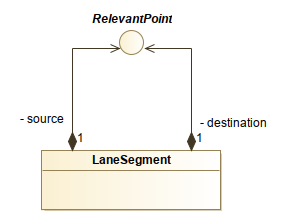
\includegraphics[scale=0.5]{img/model00}
	\caption{Entità basilari in un sistema stradale}
	\label{fig:model00}
\end{figure}

Si definisce grado di entrata in un nodo $\delta_i(v_0)$ la cardinalità del seguente insieme:
$$\{(v, v_0) \in E\}$$
Mentre il grado di uscita $\delta_o(v_0)$ è la cardinalità di:
$$\{(v_0, v) \in E\}$$

I nodi con grado di entrata o di uscita nullo hanno speciale significato in questo ambito, ovvero se dato $v_s \in V$, $\delta_i(v_s) = 0$, allora $v_s$ è un nodo di entrata nel sistema, mentre se dato $v_d \in V$, $\delta_o(v_d) = 0$, allora $v_d$ è nodo di uscita dal sistema (\ref{fig:model01}).

Siano $S$ e $D$ i rispettivi insiemi di nodi sorgente e destinazione, è stata introdotta la seguente limitazione per semplificare il lavoro di analisi:
$$v_s \in S \Rightarrow \delta_o(v_s) = 1$$
Ovvero un nodo sorgente può essere collegato ad una sola strada.\\
Questo non limita l'espressività del sistema in quanto è sufficiente dividere un nodo sorgente per ottenere la rappresentazione desiderata (\ref{fig:graph00}).
\begin{figure}[h]
	\centering
	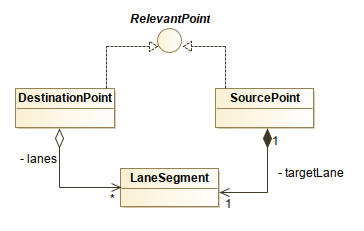
\includegraphics[scale=0.5]{img/model01}
	\caption{Sorgenti e destinazioni}
	\label{fig:model01}
\end{figure}

\begin{figure}[h]
	\centering
	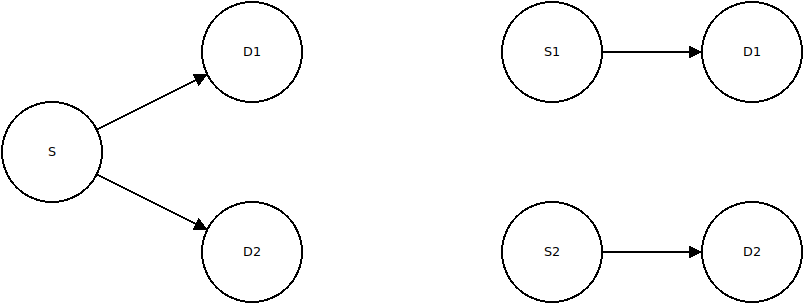
\includegraphics[scale=0.5]{img/graph00}
	\caption{Divisione di un nodo sorgente}
	\label{fig:graph00}
\end{figure}

I nodi interni alla rete invece sono realizzati da istanze della classe \textit{CrossingPoint}, che fornisce il supporto di base alla modellazione di un incrocio generico, definendo una mappa che associa ad ogni linea in entrata una o più linee in uscita: in questo modo sono coperti numerosi casi reali anche particolari, tra cui:
\begin{itemize}
	\item Impossibilità di accedere ad una strada a partire da una certa corsia.
	\item Impossibilità di effettuare inversioni ad U.
	\item Impostare alcune tratte come più o meno trafficate.
\end{itemize}

Oltre alla versione base di \textit{CrossingPoint}, che rappresenta un incrocio non arbitrato, è stata definita una versione \textit{TrafficLightCrossingPoint} che invece introduce il concetto di semaforo (\textit{TrafficLight}).
Diventa possibile associare ad ogni linea in ingresso all'incrocio un semaforo che la gestisce, in particolare sono state implementate le varianti temporizzate e a sensore: quest'ultimo caso è utile quando per esempio una linea automobilistica è interrotta da una linea tramviaria.
Vedi figura \ref{fig:model02}.

\begin{figure}[h]
	\centering
	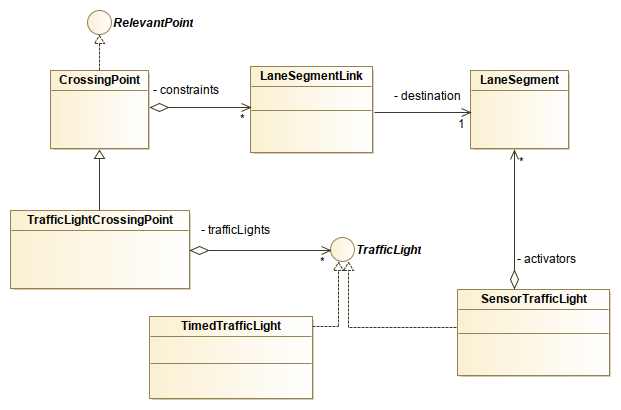
\includegraphics[scale=0.5]{img/model02}
	\caption{Modellazione di un incrocio}
	\label{fig:model02}
\end{figure}

\subsection{Configurazione}

Per gli scopi a cui è destinato, il modello mostrato non prevede particolari funzionalità operative: il suo scopo è principalmente quello di \textit{descrivere} una rete stradale.
Per poter facilmente estendere il software (per esempio con un modulo user friendly per la creazione della rete o nuove analisi non ancora previste), le entità precedentemente descritte hanno la possibilità di essere configurate con una serie arbitraria di proprietà tipizzate chiave-valore (\textit{Property}).
Sarà possibile da parte dell'utente creare una serie di proprietà e configurazioni predefinite da applicare poi ad una eventuale rete. Vedi figura \ref{fig:model03}.
Lo scopo di questo livello intermedio è quello di scaricare l'utente dalla necessità di conoscere tutte le possibili proprietà di configurazione.

\begin{figure}[h]
	\centering
	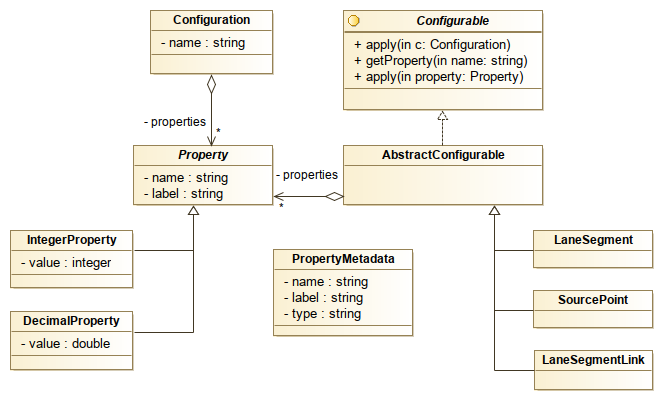
\includegraphics[scale=0.5]{img/model03}
	\caption{Configurazione}
	\label{fig:model03}
\end{figure}

La classe aggiuntiva \textit{PropertyMetadata} potrà essere utilizzata per fissare i nomi di alcune proprietà notevoli in modo da evitare errori nel tipo o nel nome al momento della definizione.



\section{Schermate dell'applicazione}
Di seguito saranno riportate alcune schermate di esempio.

\begin{figure}[h]
	\centering
	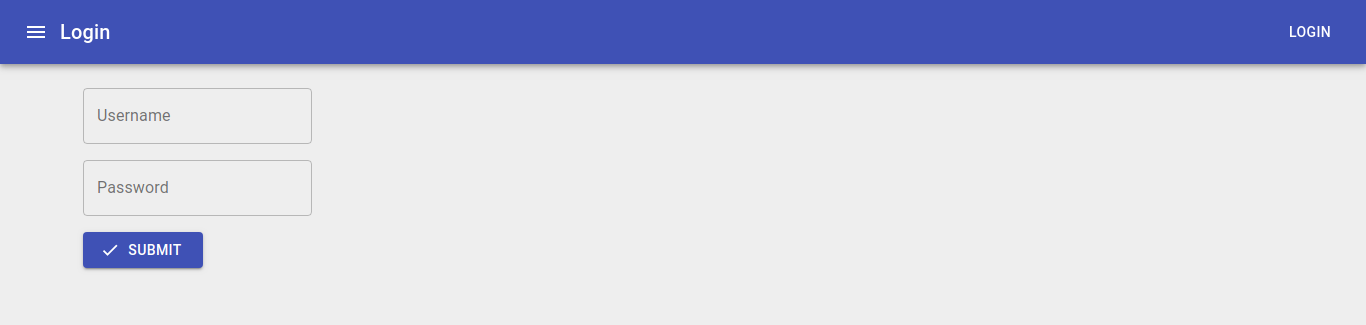
\includegraphics[width=\textwidth]{img/screen00}
	\caption{Form di login}
	\label{fig:screen00}
\end{figure}

\begin{figure}[h]
	\centering
	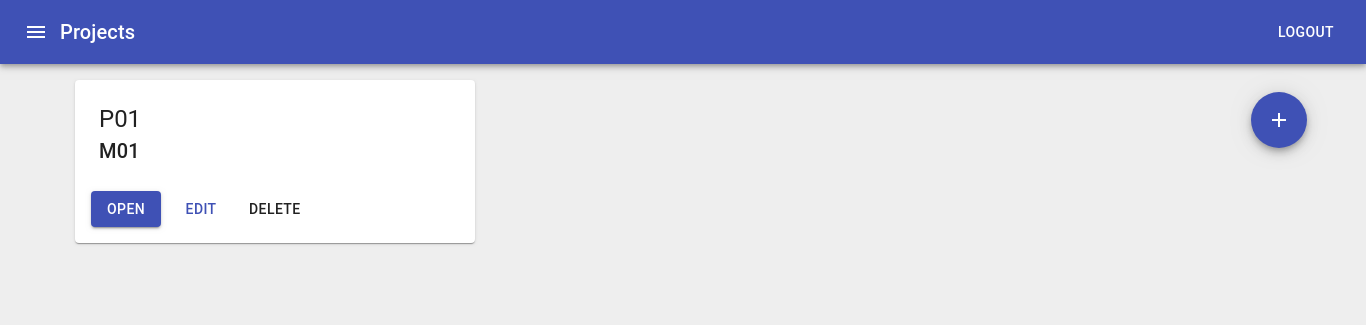
\includegraphics[width=\textwidth]{img/screen01}
	\caption{Elenco dei progetti}
	\label{fig:screen01}
\end{figure}

\begin{figure}[h]
	\centering
	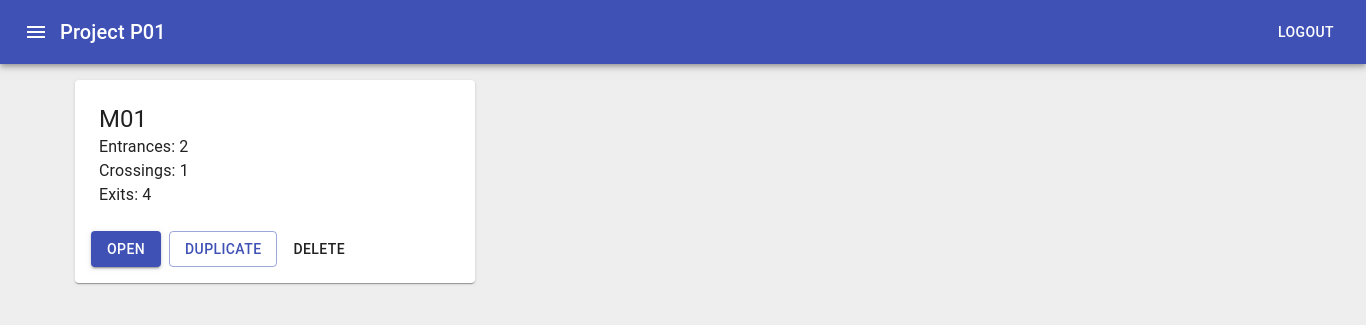
\includegraphics[width=\textwidth]{img/screen02}
	\caption{Contenuto di un progetto}
	\label{fig:screen02}
\end{figure}

\begin{figure}[h]
	\centering
	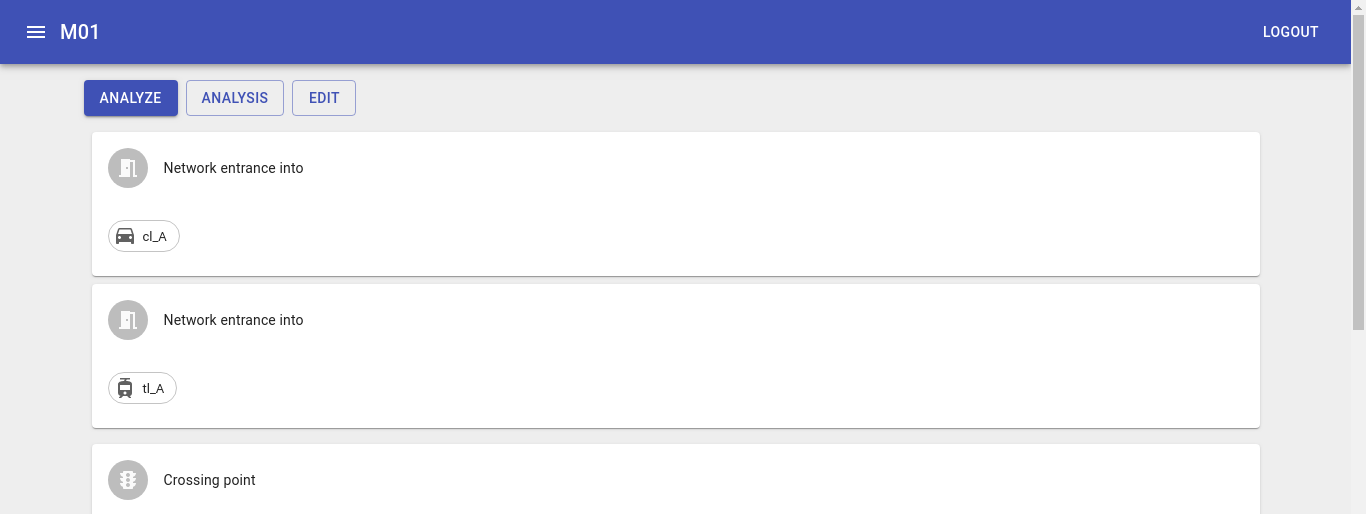
\includegraphics[width=\textwidth]{img/screen03}
	\caption{Visualizzazione di una mappa}
	\label{fig:screen03}
\end{figure}


\begin{figure}[h]
	\centering
	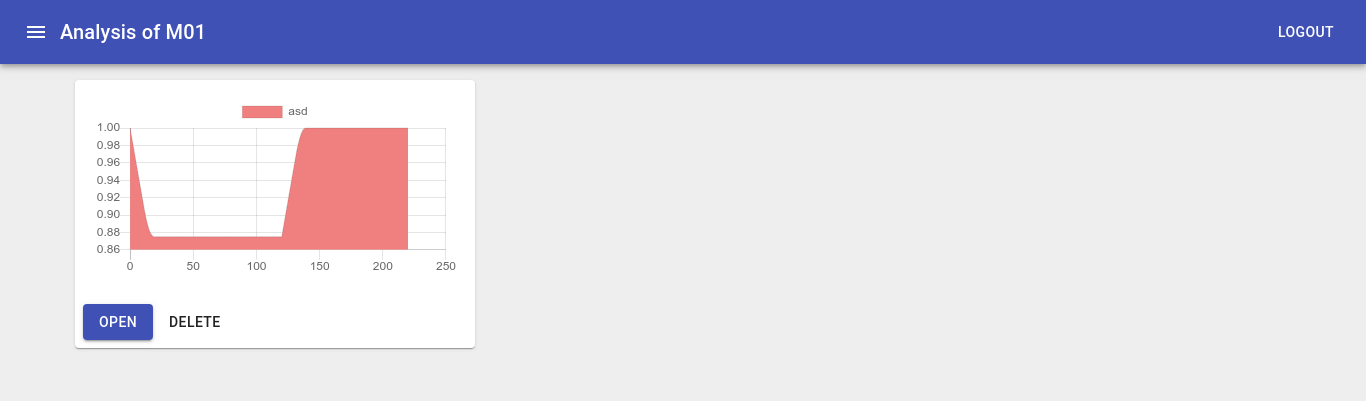
\includegraphics[width=\textwidth]{img/screen04}
	\caption{Analisi effettuate}
	\label{fig:screen04}
\end{figure}


\chapter{Architetture}

\section{Introduzione}

Il cuore di un software object-oriented si trova nel modello di dominio. Questo raccoglie i concetti estratti dall'analisi dei requisiti ed è composto da una rete di oggetti dotati di attributi e metodi che rispecchiano i \textit{dati} da memorizzare e le \textit{operazioni} necessarie alla loro elaborazione.
Questi elementi non dovrebbero avere al loro interno codice di supporto (finalizzato alla memorizzazione su un database, alla visualizzazione su interfaccia, all'invio su un canale ecc...), e in oltre questo non dovrebbe contenere frammenti di logica di dominio.
Il rischio altrimenti è quello di abbassare in maniera critica la manutenibilità del codice: le varie componenti sono accoppiate tra loro, e devono evolvere necessariamente in contemporanea.
Il test automatico diventa complesso, e si rischia di raggiungere presto lo stato di \textit{big ball of mud}\cite{microservices_architecture}.
Scrivere codice il più possibile disaccoppiato dalle tecnologie di contorno lo rende più manutenibile e testabile, ma d'altra parte può diminuire la produttività del team di sviluppo, soprattutto quando l'applicazione da sviluppare non è di eccessiva complessità.

Nel caso del lavoro corrente l'obiettivo è simulare l'evoluzione di un software da una versione monolitica ad una a microservizi: per far questo sono state sperimentate alcune architetture riconosciute, applicando quando possibile il principio di separazione delle responsabilità, fondamentale quando si parla di microservizi.

La prima architettura presa in esame è quella a livelli.

\section{Architettura a livelli}

Questo tipo di architettura è uno degli standard più affermati nello sviluppo di applicazioni enterprise.\\
Il codice è organizzato a livelli sovrapposti, ognuno dei quali può sfruttare i servizi esposti \textbf{soltanto} dai quelli sottostanti.
Esistono una serie di layers standard, di seguito se ne riportano alcuni dei più comuni\cite{ddd}:
\begin{itemize}
	\item Presentation: Fornisce informazioni e interpreta i comandi provenienti dall'esterno, in modo da interfacciarsi con un utente o un'altro software.
	\item Application: Sottile strato che dirige la logica di dominio delegando le azioni ai business objects.
	\item Model: Mantiene lo stato della logica di dominio e contiene le regole che la governano. \'E il cuore del software.
	\item Infrastructure: Fornisce funzionalità utili agli altri strati come persistenza, invio di messaggi, creazione interfaccia grafica ecc...
\end{itemize}
In questa visione il livello di business logic è consapevole dei livelli sottostanti, e può interagire direttamente con essi.
Dovendo gestire più ad alto livello la logica di dominio, per esempio aprendo e chiudendo una transazione, anche il livello application necessita di interagire con lo strato di infrastruttura.

Le linee guida per realizzare un'applicazione seguendo questa architettura prevedono di partizionare il codice in livelli coesi e dipendenti solamente da quelli sottostanti.

Esistono varie versioni di questa architettura, in cui i livelli di contorno variano: una di queste è la \textit{three layered architecture} (vedi figura \ref{fig:layered-architecture}), che prevede i livelli di \textit{Presentation} per la gestione della UI, \textit{Business Logic} per la logica di dominio e \textit{Persistence} per dialogare con i database.
Questi sono sufficienti per gran parte della applicazioni enterprise, in particolare se l'approccio usato è quello del monolite o del monolite a servizi.\\

\begin{figure}[h]
	\centering
	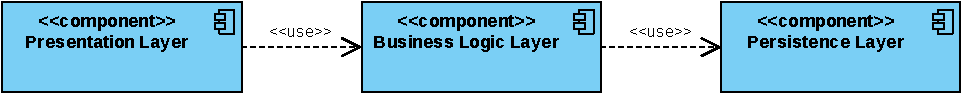
\includegraphics[width=\textwidth]{img/layered-architecture}
	\caption{Architettura a tre livelli}
	\label{fig:layered-architecture}
\end{figure}

Ogni livello può avere più istanze o essere ulteriormente separato, per esempio quando vi sono più interfacce grafiche verso la stessa applicazione, o più database che forniscono il servizio di persistenza.\\
Gli oggetti del modello di dominio devono essere, come già affermato, indipendenti dalle varie rappresentazioni, siano queste destinate ad UI, persistenza o altro.
Un indice di cattiva separazione delle responsabilità può essere per esempio la necessità di duplicare codice, o di modificare la logica di dominio quando si aggiunge una nuova interfaccia all'applicazione.\\
La separazione in layers permette inoltre di poter effettuare il rilascio delle varie parti dell'applicazione su macchine differenti, favorendone l'evoluzione e la scalabilità.
\section{Ports and adapters}

Una delle alternative all'architettura organizzata a \textit{layers} è l'architettura chiamata \textit{ports and adapters} o \textit{hexagonal architecture}\cite{microservices_architecture}.

\begin{figure}[h]
	\centering
	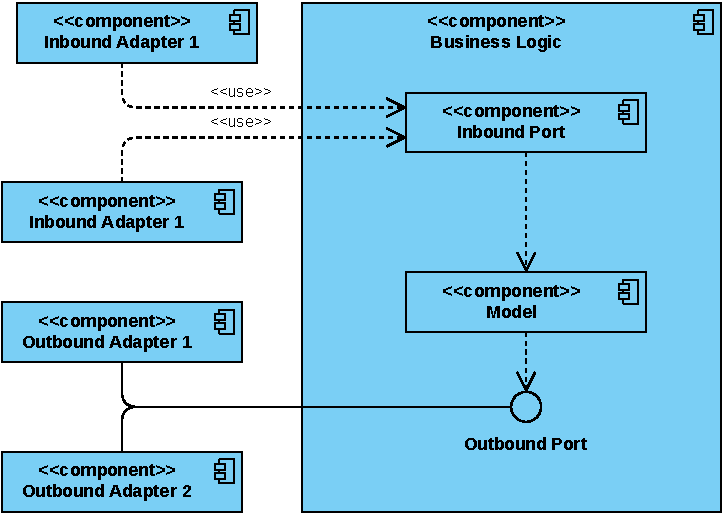
\includegraphics[width=\textwidth]{img/hexagonal-component-diagram}
	\caption{Architettura ports and adapters}
	\label{fig:hexagonal-architecture}
\end{figure}

Questo modo di organizzare i componenti del sistema è focalizzato sull'isolamento della logica di dominio.\\
Le comunicazioni di input/output con l'esterno sono guidate da interfacce \textbf{definite dal nucleo} e chiamate \textit{porte}: queste possono essere di tipo \textit{inbound} quando un modulo esterno ha necessità di invocare la logica di dominio, o di tipo \textit{outbound} quando il nucleo ha la necessità di invocare servizi esterni.
Ogni porta può avere più \textit{adattatori} associati, elementi che servono per collegare realmente i componenti esterni al nucleo.
La logica di dominio implementa le porte di tipo \textit{inbound}, che saranno usate dagli adattatori in ingresso per richiedere servizi all'applicativo.
Gli adattatori in uscita implementano le porte di tipo \textit{outbound}.

Partendo da un sistema costruito a livelli è possibile derivare l'equivalente in architettura esagonale considerando i seguenti fatti:
\begin{itemize}
	\item Se il client di un'applicazione a livelli è un'altro software, il livello di presentazione del primo può essere molto legato al livello di persistenza del secondo: ciò che è esterno alla logica di dominio quindi puòò essere visto semplicemente come un'interfaccia esterna
	\item In un'architettura a livelli moderna difficilmente la progettazione inizia dal livello di persistenza: spesso questo è realizzato da classi DAO (Data Access Object) che implementano un'interfaccia definita sulla base delle necessità del livello di business logic: questo crea una dipendenza in qualche modo inversa rispetto alla filosofia dell'architettura, enfatizzando il fatto che la logica di dominio è il centro dell'applicativo.
\end{itemize}

Rifattorizzare un progetto basato su architettura three tier per renderlo compatibile con quella ports/adapters a volte potrebbe limitarsi alla riorganizzazione dei package, senza necessitare modifiche al codice: questo perché i componenti di un'architettura a livelli spesso hanno un equivalente in architettura esagonale (vedi figura ).

Può capitare che data un'applicazione enterprise moderna
Anche in questo caso si cerca di rendere il più possibile indipendente il nucleo di un'applicazione dalle tecnologie di contorno, come database, sistema di scambio messaggi ecc...

Convertire un'applicazione service oriented realizzata a layers in una aderente all'architettura esagonale non è un'operazione complessa: se per esempio lo stack è di tipo 3-tier con una serie di servizi REST esposti che invocano internamente la logica di dominio ed uno strato di persistenza (es: JPA), il mapping è immediato (vedi figura \ref{fig:layered-hexagonal}).

\begin{figure}[h]
	\centering
	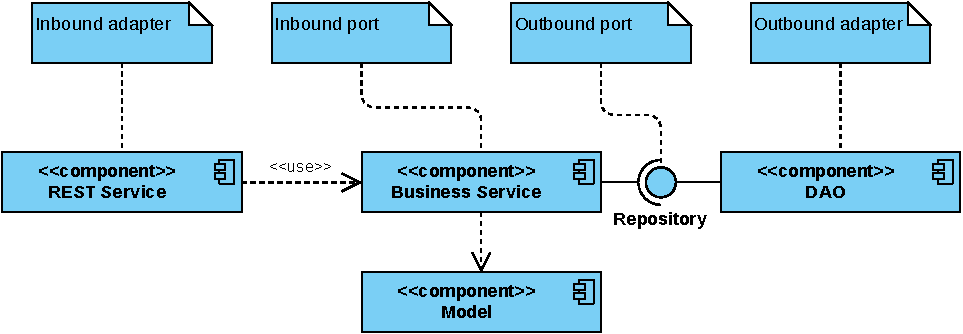
\includegraphics[width=\textwidth]{img/layered-hexagonal}
	\caption{Confronto architettura a livelli e ports/adapters}
	\label{fig:layered-hexagonal}
\end{figure}

I benefici di tale organizzazione diventano evidenti quando utilizzata all'interno di un software a microservizi, in quanto si è obbligati a identificare con chiarezza quali sono i confini del servizio, favorendo manutenibilità e testabilità.

\section{Logica di dominio}

Quando si parla di realizzare la logica di dominio per un'applicazione enterprise vi sono numerosi approcci che si possono adottare: di seguito riportiamo due patterns notevoli\cite{enterprise_app} che si contrappongono rispetto a dove verrà posta la maggior parte della logica.

\subsection{Transaction script}
La logica di dominio è posta principalmente in oggetti esterni al modello vero e proprio: il vero centro dell'applicazione è dato dai componenti chiamati \textit{Business Service} in figura \ref{fig:layered-hexagonal}.
L'idea è quella di avere entità più leggere, facilmente mappabili su un database.
Questo approccio può essere utile quando si utilizza un framework come JPA per la persistenza: si ha infatti il vantaggio di ridurre drasticamente il numero di righe di codice di tale livello, accettando il compromesso di "sporcare" le classi di modello con alcune annotazioni accoppiate ad una tecnologia.
Rendendo la separazione tra livelli o tra nucleo e porte più labile, questo approccio è adatto quando la logica di dominio non è particolarmente complessa e probabilmente non evolverà molto.

\subsection{Domain model}
La logica di dominio è contenuta quasi interamente all'interno degli oggetti del modello (\textit{Model} in figura \ref{fig:layered-hexagonal}).
Questo approccio permette di mettere in

\subsection{Architettura del software}
Il sistema è stato realizzato separando lo strato di UI da quello di business logic, realizzando secondo i principi dell'architettura \textit{ports/adapters}.\\
In particolare sono esposti verso l'esterno (inbound) una serie di servizi REST necessari all'interazione, ed è utilizzato un servizio di persistenza relazionale (outbound) necessario alla memorizzazione di informazioni come il profilo degli utenti, i progetti e le analisi effettuate.
In figura \ref{fig:architecture00} è mostrato lo schema generale.

\begin{figure}[h]
	\centering
	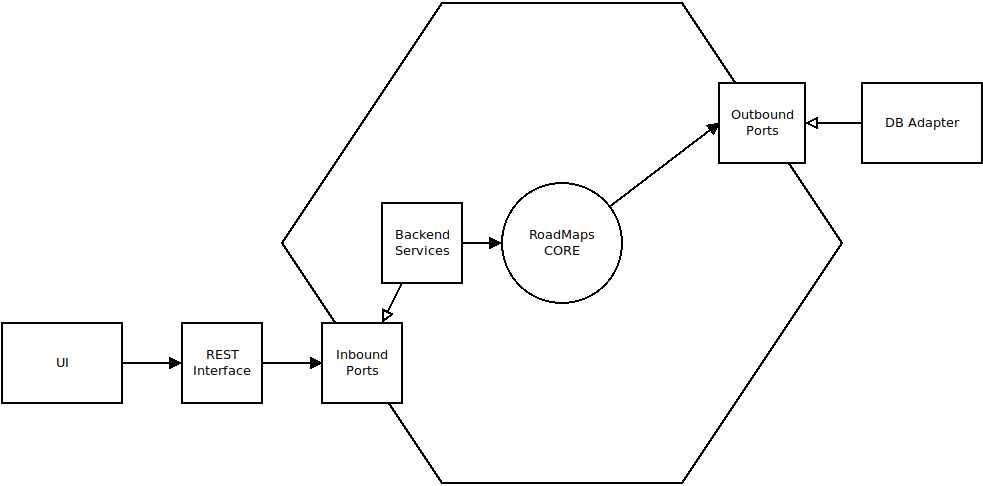
\includegraphics[width=\textwidth]{img/architecture00}
	\caption{Architettura generale}
	\label{fig:architecture00}
\end{figure}

I requisiti permettono di dividere naturalmente i servizi, le porte e gli adattatori in tre categorie:
\begin{itemize}
	\item Gestione degli utenti;
	\item Gestione delle configurazioni;
	\item Gestione dei progetti;
\end{itemize}

Un altro modulo piuttosto indipendente è quello relativo alla gestione delle analisi, ma essendo queste legate strettamente ad un progetto, saranno considerate parte dello stesso servizio.

Ognuno di questi moduli darà luogo ad un endpoint REST corrispondente ad uno o più casi d'uso, ad almeno un'entità principale e ad almeno una tabella su RDB.
Di seguito verrà riportata la descrizione di ognuno di questi blocchi partendo dal centro del modello di dominio e spostandosi all'esterno.

\subsubsection{Gestione degli utenti}
Il frammento di modello di dominio relativo alla gestione utenti è quello in figura \ref{fig:users_diagram}.

\begin{figure}[h]
	\centering
	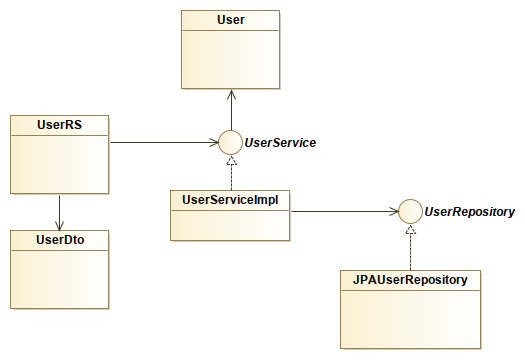
\includegraphics[width=\textwidth]{img/users_diagram}
	\caption{Diagramma delle classi relative alla gestione degli utenti}
	\label{fig:users_diagram}
\end{figure}

Dallo schema è possibile individuare quali siano le varie componenti associabili ai concetti dell'architettura esagonale:
\begin{itemize}
	\item UserService: Rappresenta una \textit{inbound port} che espone all'esterno le funzionalità relative ad un utente;
	\item UserServiceImpl: Implementa l'interfaccia \textit{UserService}, ed è quindi un \textit{inbound adapter};
	\item UserRepository: \'E una \textit{outbound port} necessaria per fornire alla logica di dominio le funzionalità di persistenza;
	\item JPAUserRepository: Implementazione di \textit{UserRepository} e quindi \textit{outbound adapter}, dipendente da una tecnologia specifica (Database relazionali + JPA), fornisce il collegamento con un RDBMS.
	\item UserRS: \'E un controller REST che espone verso il sottosistema UI i dati e le funzionalità di backend.
\end{itemize}

\subsubsection{Gestione delle configurazioni}
Il frammento di modello di dominio relativo alla gestione delle configurazioni è quello in figura \ref{fig:configurations_diagram}.

\begin{figure}[h]
	\centering
	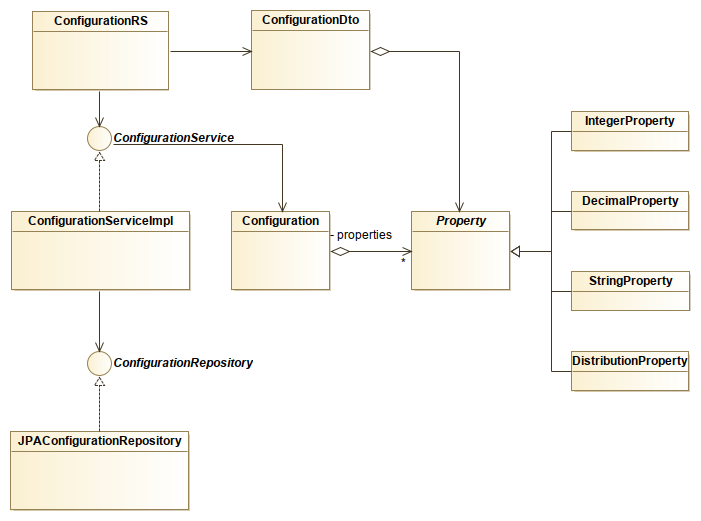
\includegraphics[width=\textwidth]{img/configurations_diagram}
	\caption{Diagramma delle classi relative alla gestione delle configurazioni}
	\label{fig:configurations_diagram}
\end{figure}

La struttura generale è equivalente a quella della sezione utenti: si hanno due interfacce \textit{ConfigurationService} e \textit{ConfigurationRepository} corrispondenti alle porte \textit{inbound} e \textit{outbound}, con i relativi adattatori \textit{ConfigurationServiceImpl} e \textit{JPAConfigurationRepository}.\\
Vi è sempre un controller REST per ricevere comandi dall'esterno del sistema, utilizzando in questo caso direttamente alcune entità del modello di dominio.

\subsubsection{Gestione dei progetti}
Il frammento di modello di dominio relativo alla gestione utenti è quello in figura \ref{fig:projects_diagram}.

\begin{figure}[h]
	\centering
	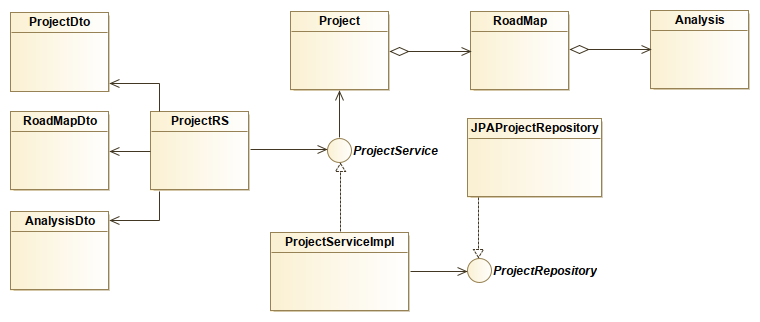
\includegraphics[width=\textwidth]{img/projects_diagram}
	\caption{Diagramma delle classi relative alla gestione dei progetti}
	\label{fig:projects_diagram}
\end{figure}

Anche in questo caso vi sono le stesse porte e adattatori più il controller REST relativo.

\chapter{Tecnologie}

TODO
\subsection{UI}

La parte di interfaccia è stata realizzata nei linguaggi HTML/CSS/JS, utilizzando in particolare il framework \textit{React}\cite{react} e la libreria di componenti per quest'ultimo \textit{Material-UI}\cite{material_ui}, che implementano le linee guide di Material Design\cite{material_design}.
%\chapter{Microservizi}

Un'architettura a microservizi è una variante dell'architettura \textit{Service oriented} che prevede di strutturare un'applicazione come un insieme di moduli disaccoppiati tra loro, indipendentemente rilasciabili, manutenibili e testabili.\\
I servizi possono comunicare tra loro tramite protocolli di vario tipo, sia sincroni che asincroni.

\section{Scalabilità}
Un'applicazione enterprise nasce naturalmente come costituita da un singolo blocco in esecuzione su di un dispositivo (fisico o virtuale).\\
I sistemi di questo tipo hanno successo quando, una volta rilasciato il software, il numero di utilizzatori rimane limitato e la manutenzione non introduce troppe nuove funzionalità.
Altrimenti, per evitare un deterioramento delle performance o eventuali fallimenti, è necessario affrontare il tema della scalabilità quando il sistema è già online, nel caso questo non sia già stato fatto in fase di progettazione.

\subsection{The Scale Cube}
In figura \ref{fig:scale_cube}\cite{the_art_of_scalability} è mostrato uno dei possibili modelli su cui è possibile lavorare per ottenere un'applicazione scalabile.
In particolare in questa rappresentazione è possibile muoversi lungo i tre assi cartesiani per ottenere scalabilità in modi diversi:

\begin{figure}[h]
	\centering
	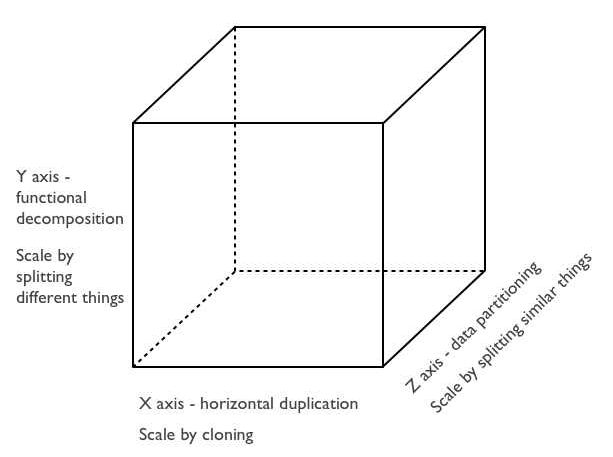
\includegraphics[scale=0.5]{img/scale_cube}
	\caption{Modulo ad architettura ports and adapters}
	\label{fig:scale_cube}
\end{figure}


\subsubsection{Asse X}
Scalare un sistema \textit{sull'asse X} significa avere più repliche della stessa applicazione in produzione; questo permette di gestire un maggior numero di richieste al secondo, eliminare i \textit{single point of failure} e non richiede grandi costi aggiuntivi di progettazione o rifattorizzazione.
Gli accessi sono gestiti da un \textit{load balancer} che avrà la responsabilità di effettuare un inoltro all'istanza più appropriata in base a vari criteri, quali zona geografica, presenza di guasti, carico di lavoro ecc...
\'E quindi possibile scegliere sistemi che operano con protocolli a vari livelli, come applicazione, trasporto o rete.
Ogni nodo potenzialmente può accedere a tutti i dati, quindi questo tipo di organizzazione non migliora i requisiti di memoria per istanza.

\subsubsection{Asse Z}
Scalare un sistema \textit{sull'asse Z} significa avere lo stesso codice replicato su più server come nel caso X, ma in questo caso ogni copia è responsabile di un sottoinsieme dei dati: il load balancer dovrà quindi inoltrare le richieste in base al contenuto di esse, operando quindi a livello applicazione.\\
Questa scelta permette di ridurre le risorse necessarie ad ogni istanza, compresa la quantità di storage o di memoria riservata alla cache.

\subsubsection{Asse Y}
Scalare un sistema \textit{sull'asse Y} significa effettuare una partizione del software per dati e/o funzionalità, partendo da un'analisi di casi d'uso e modello di dominio.\\
Si ottengono così più istanze uniche, ognuna con le proprie responsabilità ed il proprio modello di dominio.
La complessità del software viene quindi ridotta, le risorse ottimizzate la manutenibilità migliorata.\\
Questo approccio incide maggiormente sulla fase di progettazione, mentre un modo rapido per implementare questa strategia su un sistema preesistente può essere quello di replicare l'applicazione per intero come nei casi precedente e delegare ad ogni replica un particolare compito sulla base delle divisioni individuate per mezzo di un load balancer di livello applicazione.

\section{Partizionamento in microservizi}
Progettare un sistema a microservizi non è semplice quanto progettarne uno monolitico/service oriented tradizionale: difficilmente infatti un software nasce già partizionato, e a causa delle diverse complessità che questo approccio si porta dietro non è consigliabile utilizzarlo come prima carta.\\
Solitamente si sceglie di passare a tale architettura in un secondo momento, per esempio dopo molti interventi di manutenzione, quando il codice inizia ad essere troppo ampio e complesso.\cite{microservices_architecture}
In termini di scalabilità l'adottare i microservizi riguarda l'asse Y dello \textit{Scale Cube}.

Alcuni dei vantaggi principali del passare ad una architettura a microservizi sono:
\begin{itemize}
	\item Maggior facilità di manutenzione e testing.
	\item Maggiore indipendenza dei team di lavoro grazie al disaccoppiamento dei servizi.
	\item Messa in produzione indipendente.
	\item Team di sviluppo di piccole dimensioni.
\end{itemize}

\subsection{Saga}
Con il termine \textit{saga} si intende un insieme di piccole transazioni locali autoconsistenti.\\
Il coordinamento avviene in modo distribuito: ogni servizio lancerà eventi in caso di completamento o fallimento di una transazione; questi saranno quindi interpretati dagli altri moduli.\\
\'E possibile delegare le opzioni di coordinamento ad oggetti appositi.

https://microservices.io/patterns/data/saga.html

\section{Caratteristiche di un microservizio}

Temi ricorrenti quando si parla di microservizi sono quelli riguardanti la dimensione che un servizio deve avere, il numero di responsabilità, l'integrità delle informazioni ecc...\\
La linea guida principale da seguire è quella di fare in modo che i servizi siano il più possibile indipendenti tra loro, favorendo coesione, evitando un eccessivo accoppiamento.\\
Un servizio per essere tale dev'essere rilasciabile in modo indipendente dagli altri: esso infatti è l'unità minima dell'architettura. Ognuno può potenzialmente utilizzare la propria tecnologia, cosa che favorisce l'evoluzione ed evita che il software nel tempo resti legato ad una tecnologia datata.\\
Il partizionamento del monolite deve portare ad avere un certo numero di servizi disaccoppiati ma coesi: occorre studiare bene quali siano i giusti confini lungo cui tagliare il software, in modo che i nodi possano lavorare in indipendenza, ognuno con le proprie responsabilità.
%\chapter{Docker}


%\chapter{Servizi di cloud computing}\label{ch:chapter1}

\section{Software as a service}
Per \textit{software as a service} si intendono un'insieme di applicazioni accessibili al cliente tramite Internet e spesso semplicemente attraverso un browser.\\
L'utente non possiede il software ma paga per poterlo utilizzare, solitamente tramite un abbonamento o un costo a consumo.\\
I servizi sono ospitati su una piattaforma remota gestita da un provider.

\section{Platform as a service}
Per ospitare un \textit{SaaS} è possibile servirsi di una \textit{Platform as a Service}.\\
Anche in questo caso si tratta di un servizio accessibile tramite Internet, ma quella che viene offerta è una vera e propria piattaforma che fornisce un framework su cui sviluppare e caricare applicazioni.\\
Una \textit{PaaS} è rivolta agli sviluppatori, e prevedono anche in questo caso piani di pagamento a consumo o abbonamenti.
Uno dei vantaggi principali è che l'infrastruttura sottostante è condivisa con altri utenti, cosa che limita il costo del servizio.

\section{Infrastructure as a service}
Quando si necessita di un maggior controllo e flessibilità è possibile affidarsi ad una soluzione \textit{Infrastructure as a service}.
In questo caso il cliente può arrivare a gestire l'intero sistema operativo senza comunque preoccuparsi della livello hardware sottostante.
%\chapter{Conclusioni}\label{ch:conclusioni}
\ldots

\addcontentsline{toc}{chapter}{Bibliografia}
\bibliographystyle{plain}
\bibliography{files/biblio}
%\bibliographystyle{unsrt}
%\bibliography{sp,xml}

\end{document}